\subsection{域的可分闭包}

定义 4.——称域 K 是可分封闭的，如果 K 的每个可分代数扩张都是平凡的。

代数闭域是可分封闭的。反之，若完全域 K 是可分封闭的，则它是代数闭的，因为 K 的每个代数扩张都可分（V，第 3 页，命题 2）。

定义 5.——设 K 是一个域。所谓 K 的可分代数闭包，或（出于用语之便）K 的可分闭包，是指 K 的这样一个扩张 E：它在 K 上代数且可分，并且域 E 本身是可分封闭的。

当 K 为完全域时，K 的可分闭包与代数闭包这两个概念完全同一（V，第 36 页，命题 2 及第 43 页，推论 1）。

命题 14.——设 \(\Omega\) 是 K 的一个代数闭扩张。

\begin{enumerate}
\def\labelenumi{\alph{enumi})}
\item
  相对可分代数闭包 \(\Omega_s\) （\(\mathbf{K}\) 在 \(\Omega\) 中的）是 \(\mathbf{K}\) 的一个可分闭包。
\item
  若 E 与 E' 是 K 的两个可分闭包，则存在 E 到 E' 上的一个 K-同构。
\end{enumerate}

设 \(F\) 是 \(\Omega_s\) 的一个可分代数扩张；由于 \(\Omega\) 代数闭，存在 \(\Omega_s\) -同态 \(u\) 将 \(F\) 映入 \(\Omega\) （V，第 20 页，定理 1）。由命题 9（V，第 42 页），\(u(F)\) 在 \(K\) 上可分，因此 \(u(F) = \Omega_s\) 。于是 \(F\) 是 \(\Omega_s\) 的平凡扩张，故 \(\Omega_s\) 可分封闭，由此得 \(a\) ).

设 E 是 K 的一个可分闭包。由于 E 是 K 的代数扩张，故存在 E 到 \(\Omega\) 中的 K-同态 v（V，第 20 页，定理 1）。于是 \(v(\mathrm{E})\) 在 K 上是可分代数的，从而 \(v(\mathrm{E}) \subset \Omega_{s}\) 。由 V，第 42 页命题 9，\(\Omega_{s}\) 在 \(v(\mathrm{E})\) 上可分；又因域 \(v(\mathrm{E})\) 可分封闭，我们有 \(v(\mathrm{E}) = \Omega_{s}\) 。由此可知，v 是 E 到 \(\Omega_{s}\) 上的 K-同构。于是 b) 是直接推论。

推论.——设 E 是 K 的一个可分封闭扩张，F 是 K 的一个可分代数扩张；则存在 F 到 E 中的 K-同态。

设 \(\Omega\) 是 E 的一个代数闭包；我们有 \(\Omega_s \subset E\) ，于是只需处理 \(E = \Omega_s\) 的情形。由于 F 是 K 的代数扩张，存在 K-同态 \(u\) 将 F 映入 \(\Omega\) （V，第 20 页，定理 1）。由于域 \(u(F)\) 在 K 上可分，我们有 \(u(F) \subset \Omega_s\) ，且 \(u\) 定义了 F 到 \(\Omega_s = E\) 中的 K-同态。

\pandocbounded{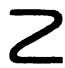
\includegraphics[keepaspectratio]{images/part001_42ca6df9.jpg}}

注记.—— 1) 设 E 与 E' 是 K 的两个可分闭包。若 K 不是可分封闭的，则存在多个 E 到 E' 上的 K-同构。因为此时 E 是 K 的非平凡伽罗瓦扩张，故存在异于恒等映射的 E 的 K-自同构（V，第 56 页，定理 1）。

2) 设 \(E\) 是 \(K\) 的一个代数可分扩张。若 \(K\) 的每个代数且可分的扩张都同构于 \(E\) 的一个子扩张，则 \(E\) 是 K 的一个可分闭包。因为若 \(E'\) 是 K 的一个可分闭包，则扩张 E 与 \(E'\) 中的每一个都同构于另一个的子扩张；因此 E 与 \(E'\) 是 K 的同构扩张（V，第 52 页，命题 1，a)）。

